\documentclass{article}
\usepackage[a4paper, left=0.5in, right=0.4in, top=0.5in, bottom=0.5in]{geometry}
\usepackage{xparse}
\usepackage{float}
\usepackage{hyperref}
\usepackage{cite}
\usepackage{graphicx}
\usepackage{adjustbox}
\usepackage{enumitem}
\usepackage{amsmath, amssymb}
\usepackage{tikz}
\usepackage{tikz-timing}[2014/10/29]
\usepackage{bytefield}
\usepackage{multirow}
\usepackage{xcolor}
\usepackage{rotating}

\usetikztiminglibrary[rising arrows]{clockarrows}

\NewDocumentCommand{\busref}{som}{\texttt{%
		#3%
		\IfValueTF{#2}{[#2]}{}%
		\IfBooleanTF{#1}{\#}{}%
}}

\newcommand{\bitlabel}[2]{%
\bitbox[]{#1}{%
\raisebox{0pt}[2ex][0pt]{%
\turnbox{45}{\fontsize{7}{7}\selectfont#2}%
}%
}%
}

\title{USB - A Study}
\author{Narendiran S}
\date{03-07-2021}

\begin{document}
\Large
\maketitle
\section{Source: Dogan Ibrahim - Advanced PIC Microcontroller Projects in C From USB to RTOS with the PIC 18F Series (2008, Newnes)}

\begin{itemize}
    \item By USB Implementation Forum Inc. (Compaq, Microsfot, Intel, NECT, HP, Lucent, Philips, etc.)
    \item High-sepped Serial interface
    \item 127 devices (7-bit address filed -- Address 0 is reserverd)
    \item Thirty meters max
    \item Maximum tiers (hubs) can be 6
    \item USB 1.1 -- 11 Mbps \& USB 2.0 -- 480 Mbps
          \begin{itemize}
              \item Low Speed - 1.5 Mbps
              \item Full Speed - 12 Mbps
              \item High Speed - 480 Mbps
          \end{itemize}
    \item White $--$ Data- \& Green $--$ Data+ carry differential data signals and signle-ended data states.
    \item USB signals are bi-phase and uses NRZI (Non-Return to Zero Inverted) data encoding.
    \item{NRZI}
          \begin{itemize}
              \item Uses clock.
              \item If the data bit is 1, the NRZI transitions at clock boudaries.
              \item If the data bit is 0, no transitions.
              \item NRZI may have long series of 0s or 1s, resulting in clock recovery difficulties.
          \end{itemize}
          \begin{center}
              \begin{tikztimingtable}[%
                      timing/dslope=0.1,
                      timing/.style={x=5ex,y=2ex},
                      x=5ex,
                      timing/rowdist=3ex,
                      timing/c/rising arrows,
                      timing/name/.style={font=\sffamily\scriptsize}
                  ]
                  \busref{CLK}         & 2{l} 26{c} \\
                  \busref{DATA} & D{0}; D{1}; D{1}; D{1}; D{1};  D{0}; D{0}; D{1}; D{0}; D{0}; D{0}; D{0}; D{1};D{0};\\
                  \busref{NRZI} & h h; L; H; L; H; H; H; L; L; L; L; L; H; H;\\
                  \extracode
                  \begin{pgfonlayer}{background}
                      \begin{scope}[semitransparent,semithick]
                          \vertlines[red]{1,2,...,7}
                      \end{scope}
                  \end{pgfonlayer}
              \end{tikztimingtable}
          \end{center}
    \item NRZI may have long series of 0s or 1s, resulting in clock recovery difficulties.
    \item Hence, a concept of \verb|bit stuffing| is used where after every six consecutive ones, a 0 bit is stuffed.
    \item Packet of data transmitted by host is sent to every device connected  to the bus.
    \item All the devices receive the signal, but only the addressed one accepts the data.
    \item Only one device can transmit data to the host.
    \item Device class - enables same device driver to be used for several devices having similar functionalities.
    \item{Device Class}
          \begin{table}[H]
              \centering
              \begin{tabular}{|c|c|c|}
                  \hline
                  \textbf{Device Class} & \textbf{Description}         & \textbf{Example Devices} \\
                  \hline
                  0x00                  & Reserved                     & -                        \\
                  \hline
                  0x01                  & USB Audio Device             & Sound Card               \\
                  \hline
                  0x02                  & USB Communications Device    & Modem, Fax               \\
                  \hline
                  0x03                  & USB Human Interface Device   & Keyboard, Mouse          \\
                  \hline
                  0x07                  & USB Printer Device           & Printer                  \\
                  \hline
                  0x08                  & USB Mass Storage Device      & Memory Card, Flash Drive \\
                  \hline
                  0x09                  & USB Hub Device               & Hubs                     \\
                  \hline
                  0x0B                  & USB Smart Card Reader Device & Card Reader              \\
                  \hline
                  0x0E                  & USB Video Device             & Webcam, Scanner          \\
                  \hline
                  0xE0                  & USB Wireless Device          & Bluetooth                \\
                  \hline
              \end{tabular}
          \end{table}
    \item Commom USB Terms
          \begin{itemize}
              \item Endpoint -  Either a source or a sink of data. A single USB device can have sixteen IN endpoints and sixteen OUT endpoints.
              \item Trasactions - transfer of data on the bus.
              \item Pipe - Logic data connection between the host and an endpoint.
          \end{itemize}
\end{itemize}



\subsection{Speed and Device plugged Identification on Bus}
\label{sec: deviIden}
\begin{itemize}
    \item At the device end (client side or endpoint) of the bus, a 1.5K pull-up resistor is connected from D+ or D- to 3.3V.
    \item For full-speed bus, D+ line is pulled to 3.3V through pull-up resistor.
    \item For Low-speed bus, D- line is pulled to 3.3V through pull-up resistor.
    \item When no device is plugged, the host sees a low on the data lines.
    \item When a device is plugged in, either of the D+ or D- is pulled high, and the host knows that a devie is plugged into the bus.
    \item The speed is determined by with line is pulled high.
\end{itemize}

\subsection{USB States}
\begin{table}[H]
    \begin{center}
        \begin{tabular}{|c|p{5cm}|p{10cm}|}
            \hline
            \textbf{USB States} & \textbf{Line Values (D+ and D-)}                                                                                                                                & \textbf{Description}                                                                                                                                                \\
            \hline
            \hline
            \textbf{IDLE}       & Bus in idle state, one line is high and other line is low (which line is high and which line is low depends on the speed mode(See Section \ref{sec: deviIden})) & This is the state of lines before and after a packet transmission. Also, the device is plugged in.                                                                  \\
            \hline
            \textbf{DETACHED}   & Both lines are low.                                                                                                                                             & No devices is plugged/connected.                                                                                                                                    \\
            \hline
            \textbf{ATTACHED}   & Either of the line is logic high.                                                                                                                               & Devices is plugged/connected.                                                                                                                                       \\
            \hline
            \textbf{J State}    & Same as idle                                                                                                                                                    & Same as idle                                                                                                                                                        \\
            \hline
            \textbf{K State}    & Opposite of J State                                                                                                                                             & Opposite of J State                                                                                                                                                 \\
            \hline
            \textbf{SE0}        & Single Ended Zero State, both lines are pulled low                                                                                                              & -                                                                                                                                                                   \\
            \hline
            \textbf{SE1}        & Single Ended One State, both lines are pulled high                                                                                                              & Illegal condition, should never happen                                                                                                                              \\
            \hline
            \textbf{RESET}      & pulling both the lines low (SE0 State) for at least 10ms.                                                                                                       & When host wants to communicate with device on bus, it first sends a reset condition.                                                                                \\
            \hline
            \textbf{EOP}        & -                                                                                                                                                               & End of Packet state - SE0 state for 2 bit times, followed by J State for 1 bit time.                                                                                \\
            \hline
            \textbf{KEEP ALIVE} & -                                                                                                                                                               & Keep Alive State is achieved after EOP State. Keep Alive is sent at least once every millisecond to keep the device from suspending.                                \\
            \hline
            \textbf{SUSPEND}    & -                                                                                                                                                               & Used to Save Power, Suspend is done by not sendingy anything to a device for 3ms. Suspended device draws less than 0.5mA and must recognie reset and resume signal. \\
            \hline
            \textbf{RESUME}     & Reversing the polarity of the singal on the data lines for at leaset 20ms followed by a low-speed EOP signal                                                    & Suspended device is woken using resume by sending resersed polrity signal for 20 ms and then low-speed EOP                                                          \\
            \hline
        \end{tabular}
    \end{center}
\end{table}

\subsection{USB Bus Communication}
\begin{itemize}
    \item USB is host-centric connectivity system, so host dictates the use of USB Bus.
    \item Each device on the bus is assigned a unique USB address.
    \item No slave device can assert signal on the bus, until the host asks for it.
\end{itemize}

\subsubsection{Initial Operation}
\begin{enumerate}[label=\roman*)]
    \item A new device is plugged in is identified by either of D+ or D- line going high (Generally both lines are low).
    \item When new device is blugged into bus, the USB host uses the address 0 to ask basic information from the device.
    \item Then, host assigns unique USB address.
    \item Then, host ask for and gets infomations such as name of manufacturer, device capacilities, product ID, etc.
    \item Then two-way transactions on the bus can begin.
\end{enumerate}

\subsection{Packets}
\begin{itemize}
    \item Data is transmitted on a USB bus using Packets.
    \item A packet starts with a 8-bit sync pattern to allow receiver clock to synchronize with the data.
    \item Followed by the \textbf{Packet Identifier (PID)} byte information.
          \begin{itemize}
              \item PID byte is a 8-bit long.
              \item PID is 4bit + 4-bit coplemented PID.
              \item Based on the which PID, four packes are available : \textit{Token, Data, Handshake, Special}
          \end{itemize}
          \begin{table}[H]
              \centering
              \begin{tabular}{|c|c|c|p{9cm}|}
                  \hline
                  \textbf{PID type - Packet}        & \textbf{Bits}                   & \textbf{PID name} & \textbf{Description}                                                 \\
                  \hline
                  \multirow{4}{*}{Data Packet}      & 11\textcolor{magenta}{00}\_0011 & DATA0             & Data Packet PID even                                                 \\
                                                    & 01\textcolor{magenta}{00}\_1011 & DATA1             & Data Packet PID odd                                                  \\
                                                    & 10\textcolor{magenta}{00}\_0111 & DATA2             & Data Packet PID high speed                                           \\
                                                    & 00\textcolor{magenta}{00}\_1111 & MDATA             & Data Packet PID high speed                                           \\
                  \hline
                  \multirow{4}{*}{Handshake Packet} & 11\textcolor{magenta}{01}\_0010 & ACK               & Receiver accepts packet (Receiver acknowledges that it has received) \\
                                                    & 01\textcolor{magenta}{01}\_1010 & NAK               & Receiver did not accepts packet (Receiver cannot accept the packet)  \\
                                                    & 10\textcolor{magenta}{01}\_0110 & NYET              & No response from receiver                                            \\
                                                    & 00\textcolor{magenta}{01}\_1110 & STALL             & Stalled (Indicates endpoint is halted)                               \\
                  \hline
                  \multirow{4}{*}{Token Packet}     & 11\textcolor{magenta}{10}\_0001 & OUT               & Host to device transaction                                           \\
                                                    & 01\textcolor{magenta}{10}\_1001 & IN                & Device to host transaction                                           \\
                                                    & 10\textcolor{magenta}{10}\_0101 & SOF               & Start of frame                                                       \\
                                                    & 00\textcolor{magenta}{10}\_1101 & SETUP             & Setup Command                                                        \\
                  \hline
                  \multirow{4}{*}{Special Packet}   & 11\textcolor{magenta}{11}\_0000 & Reserved          & Reserved                                                             \\
                                                    & 01\textcolor{magenta}{11}\_1000 & SPLIT             & High-speed split transaction                                         \\
                                                    & 10\textcolor{magenta}{11}\_0100 & PING              & High-speed flow control                                              \\
                                                    & 00\textcolor{magenta}{11}\_1100 & ERR               & Split transaction error                                              \\
                                                    & 00\textcolor{magenta}{11}\_1100 & PRE               & Host preample                                                        \\
                  \hline
              \end{tabular}
          \end{table}
    \item Followed by
          \begin{itemize}
              \item 0-1024 bytes of data, 2-byte CRC checksum in case of \textit{Data Packet}.
              \item 7-bit address, a 4-bit ENDP (Endpoint Number) and a  5-bit CRC checksum in case of \textit{Token Packet}.
              \item Nothing in case of \textit{Handshake Packet}.
          \end{itemize}
    \item Finally, ends with the end of packet (EOP) signal.
\end{itemize}

\begin{table}[H]
    \centering
    \caption{Data Packet}
    \begin{tabular}{|c|c|c|c|c|}
        \hline
        \textbf{SYNC} & \textbf{PID} & \textbf{DATA} & \textbf{CRC} & \textbf{EOP} \\
        \hline
        8-bits        & 4+4 bits     & 0-1024 bytes  & 16-bits      & -            \\
        \hline
    \end{tabular}
\end{table}

\begin{table}[H]
    \centering
    \caption{Token Packet}
    \begin{tabular}{|c|c|c|c|c|c|}
        \hline
        \textbf{SYNC} & \textbf{PID} & \textbf{ADDR} & \textbf{ENDP} & \textbf{CRC} & \textbf{EOP} \\
        \hline
        8-bits        & 4+4 bits     & 7-bits        & 4-bits        & 5-bits       & -            \\
        \hline
    \end{tabular}
\end{table}

\begin{table}[H]
    \centering
    \caption{Handshake Packet}
    \begin{tabular}{|c|c|c|}
        \hline
        \textbf{SYNC} & \textbf{PID} & \textbf{EOP} \\
        \hline
        8-bits        & 4+4 bits     & -            \\
        \hline
    \end{tabular}
\end{table}


\subsection{Data Flow Types}
Data is transferred in a USB using
\begin{enumerate}
    \item Bulk transfer
    \item Interrupt transfer
    \item Isochronous transfer
    \item Control transfer
\end{enumerate}

\subsubsection{Bulk Transfer}
\begin{itemize}
    \item Transfer lare amounts of data with no errors
    \item No guarantee of bandwidth
    \item If an endpoint is defined as OUT and uses bulk tranfer.
          \begin{itemize}
              \item Then host transfer data from host to endpoint.
          \end{itemize}
    \item If an endpoint is defined as IN and uses bulk tranfer.
          \begin{itemize}
              \item Then host transfer data from endpoint to host.
          \end{itemize}
    \item Used when slow data rate is not an issue.
    \item No bulk transfer at low speed
    \item 8-64 packets at full speed
    \item 512 packets at high speed
\end{itemize}

\subsubsection{Interrupt Transfer}
\begin{itemize}
    \item Transfer small amount of data with high bandwidth.
    \item 1-8 bytes at low speed
    \item 1-64 byutes packets at full speed
    \item upto 1024 bytes at high speed
\end{itemize}

\subsubsection{Isochronous Transfer}
\begin{itemize}
    \item Guaranteed bandwidth with no guaranteed error-free
    \item Audio data (where speed is important but loss of data is not importnat)
    \item No Isochronous transfer at low speed
    \item 1023 bytes at full speed
    \item 1024 bytes at high speed
\end{itemize}

\subsubsection{Control Transfer}
\begin{itemize}
    \item Bidirectional Data transferred
    \item using both IN and OUT endpoints.
    \item for initial configuation of device by host.
    \item 8-bytes at low Speed
    \item 8-64 bytes full Speed
    \item 64-bytes at high speed.
\end{itemize}

\subsection{Enumeration}
When a device is plugged into a USB bus, it is known to the host through \textbf{Enumeration}.
The initial communication between the host and the device is carried out using the \emph{control transfer} type of data flow.



\begin{itemize}
    \item When a device is plugged in, the host becomes aware of it because one of thedata lines (D+ or D-) becomes logic high.
    \item The host sends a USB reset signal to the device to place the device in a known state.
    \item The reset device responds to address 0.
    \item The host sends a request on address 0 to the device to find out its maximum packet size using a \emph{Get Descriptor} command.
    \item The device responds by sending a small portion of the device descriptor.
    \item The host sends a USB reset again.
    \item The host assigns a unique address to the device and sends a \emph{Set Address} request to the device.
    \item After the request is completed, the device assumes the new address. At this point the host is free to reset any other newly plugged-indevices on the bus.
    \item The host sends a \emph{Get Device Descriptor} request to retrieve the complete device descriptor, gathering information such as manufacturer, type of device, and maximum control packet size.
    \item The host sends a \emph{Get Configuration Descriptors} request to receive the device’s configuration data, such as power requirements and the types and number of interfaces supported.
    \item The host may request any additional descriptors from the device.
\end{itemize}

Initially, the device is addressed, but it is in an unconfigured state.
After the host gathers enough information about the device, it loads a suitable device driver which configures the device by sending it a \emph{Set Configuration} request.
At this point the device has been configured, and it is ready to respond to device-specific requests.

\subsection{Descriptors}
All USB devices have a hierarchy of descriptors that describe various features of the device: the manufacturer ID, the version of the device, the version of USB it supports, what the device is, its power requirements, the number and type of endpoints, and so forth.
The commonly used descriptors are
\begin{itemize}
    \item Device descriptors
    \item Configuration descriptors
    \item Interface descriptors
    \item HID descriptors
    \item Endpoint descriptors
\end{itemize}

The hierarchy can be seen below
\begin{figure}[H]
    \begin{center}
        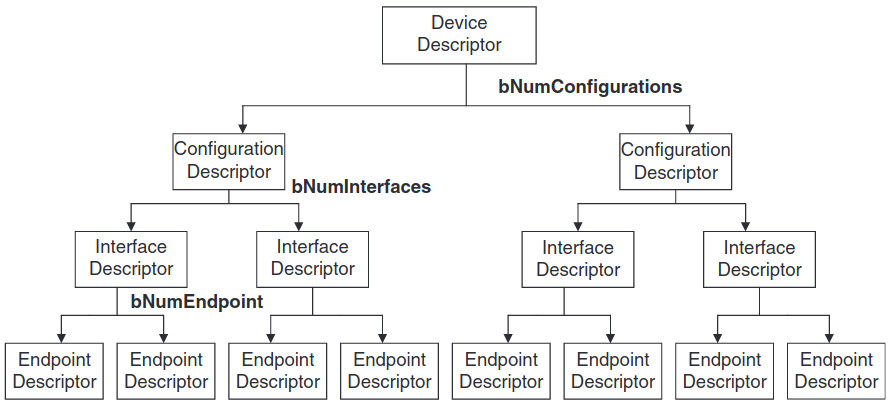
\includegraphics[scale=0.5]{DocuResources/DescriptorHierarchy.png}
    \end{center}
\end{figure}
The HID descriptor comes in same level as Interface descriptor when interface belogs to HID class.

The first byte of all descriptor is the \textit{bLength} - length of descriptor.
The second byte of all descriptor is the \textit{bDescriptorType} - type of descriptor.

\subsubsection{Device Descriptor}
\begin{itemize}
    \item Top-level information read from device.
    \item First item, the host retrieves
    \item USB device has only one Device Descriptor
    \item Represents entier device
    \item information such as manufacturer, serial number, product number, the class of the device, and the number of configurations
\end{itemize}


\begin{table}[H]
    \centering
    \begin{adjustbox}{max width=\textwidth}
        \begin{tabular}{|c|c|c|c|p{6cm}|}
            \hline
            \textbf{Offset (in Bytes)} & \textbf{Field}     & \textbf{Size (in Bytes)} & \textbf{Meaning}                   & \textbf{Description}                                                                                                                         \\
            \hline
            0                          & bLength            & 1                        & Descriptor Size in bytes           & Provides the length of this device descriptor in bytes.                                                                                      \\
            \hline
            1                          & bDescriptorType    & 1                        & Device Descritor type              & Value is 0x01 since, the type is device descriptor.                                                                                          \\
            \hline
            2                          & bcdUSB             & 2                        & Highest version of USB supported   & Provides the highest usb version supported by the device in BCD format, 0xJJMN (JJ - major version, M - minor version, N - subminor version) \\
            \hline
            4                          & bDeviceClass       & 1                        & Class Code                         & \multirow{3}{6cm}{assigned by the USB organization and used by system to find a class driver for device.}                                    \\
            \cline{1-4}
            5                          & bDeviceSubClass    & 1                        & Subclass code                      &                                                                                                                                              \\
            \cline{1-4}
            6                          & bDeviceProtocol    & 1                        & Protocol code                      &                                                                                                                                              \\
            \hline
            7                          & bMaxPacketSize0    & 1                        & Maximum Packet size                & For Endpoint 0, maximum input and output packet size                                                                                         \\
            \hline
            8                          & idVendor           & 2                        & Vendor ID                          & Vendor's ID assigned by USB organization                                                                                                     \\
            \hline
            10                         & idProduct          & 2                        & Product ID                         & Product's ID assigned by manufacturer                                                                                                        \\
            \hline
            12                         & bcdDevice          & 2                        & Device release number              & Deivce release number - same format as bcdUSB                                                                                                \\
            \hline
            14                         & iManufacturer      & 1                        & Manufacturer string descripto      & \multirow{3}{6cm}{details about the manufacturer andthe product. These fields have no requirement and can be set to zero.}                   \\
            \cline{1-4}
            15                         & iProduct           & 1                        & Index of product string descriptor &                                                                                                                                              \\
            \cline{1-4}
            16                         & iSerialNumber      & 1                        & Index of serial number descriptor  &                                                                                                                                              \\
            \hline
            17                         & bNumConfigurations & 1                        & Number of possible configurations  & Number of configuation the device supports                                                                                                   \\
            \hline
        \end{tabular}
    \end{adjustbox}
\end{table}

\subsubsection{Configuration Descriptors}
\begin{itemize}
    \item information about power requirements of the device, how many different interfaces it support
    \item may have more than one configuration for a device
    \item When the configuration descriptor is read by the host, it returns the entire configuration information, which includes all interface and endpoint descriptors.
\end{itemize}


\begin{table}[H]
    \centering
    \begin{adjustbox}{max width=\textwidth}
        \begin{tabular}{|c|c|c|c|p{6cm}|}
            \hline
            \textbf{Offset (in Bytes)} & \textbf{Field}      & \textbf{Size (in Bytes)} & \textbf{Meaning}                      & \textbf{Description}                                                                                                                   \\
            \hline
            0                          & bLength             & 1                        & Descriptor Size in bytes              & Provides the length of this configuation descriptor in bytes.                                                                          \\
            \hline
            1                          & bDescriptorType     & 1                        & Device Descritor type                 & Value is 0x02 since, the type is configuation descriptor.                                                                              \\
            \hline
            2                          & wTotalLength        & 2                        & Total bytes returned                  & total combined size of this set of descriptors (configuration descriptor + interface descriptor + HID descriptor + endpointdescriptor) \\
            \hline
            4                          & bNumInterfaces      & 1                        & Number of interfaces                  & number of interfaces present for this configuration                                                                                    \\
            \hline
            5                          & bConfigurationValue & 1                        & Value used to select configuration    & used by the host (in command SetConfiguration) to select the configuration.                                                            \\
            \hline
            6                          & iConfiguration      & 1                        & Index describing configuration string & index to a string descriptor describing the configuration inreadable format.                                                           \\
            \hline
            7                          & bmAttributes        & 1                        & Power supply attributes               & D7==1 -- Bus-powered, D6==1 -- Self Powered, D5==1 -- Remote wakeup                                                                    \\
            \hline
            8                          & bMaxPower           & 2                        & Max power consumption in 2mA          & maximum power the device will draw from the bus in 2mAunits.                                                                           \\
            \hline
        \end{tabular}
    \end{adjustbox}
\end{table}

\subsubsection{Interface Descriptors}
\begin{itemize}
    \item Specify the class of interface and the Number of endpoint it uses
    \item May be more then one interface.
\end{itemize}

\begin{table}[H]
    \centering
    \begin{adjustbox}{max width=\textwidth}
        \begin{tabular}{|c|c|c|c|p{6cm}|}
            \hline
            \textbf{Offset (in Bytes)} & \textbf{Field}     & \textbf{Size (in Bytes)} & \textbf{Meaning}                        & \textbf{Description}                                                                      \\
            \hline
            0                          & bLength            & 1                        & Descriptor Size in bytes                & Provides the length of this interface descriptor in bytes.                                \\
            \hline
            1                          & bDescriptorType    & 1                        & Device Descritor type                   & Value is 0x04 since, the type of this interface descriptor.                               \\
            \hline
            2                          & bInterfaceNumber   & 1                        & Number of interface                     & index of this interface descriptor                                                        \\
            \hline
            3                          & bAlternateSetting  & 1                        & Value to select alternate setting       & pecify alternate interfaces that can be selected by the host using command Set Interface. \\
            \hline
            4                          & bNumEndpoints      & 1                        & Number of endpoints                     & number of endpoints used by this interface.                                               \\
            \hline
            5                          & bInterfaceClass    & 1                        & Class code                              & \multirow{3}{6cm}{assigned by USB organization}                                           \\
            \cline{1-4}
            6                          & bInterfaceSubClass & 1                        & subclass code                           &                                                                                           \\
            \cline{1-4}
            7                          & bInterfaceProtocol & 1                        & protocol code                           &                                                                                           \\
            \hline
            8                          & iInterface         & 1                        & Index of string descriptor to interface & index to a string descriptor of the interface.                                            \\
            \hline
        \end{tabular}
    \end{adjustbox}
\end{table}

\subsubsection{HID Interface}
An HID descriptor always follows an interface descriptor when the interface belongs tothe HID class.
\begin{table}[H]
    \centering
    \begin{adjustbox}{max width=\textwidth}
        \begin{tabular}{|c|c|c|c|p{6cm}|}
            \hline
            \textbf{Offset (in Bytes)} & \textbf{Field}    & \textbf{Size (in Bytes)} & \textbf{Meaning}                 & \textbf{Description}                                                        \\
            \hline
            0                          & bLength           & 1                        & Descriptor Size in bytes         & Provides the length of this  HID descriptor in bytes.                       \\
            \hline
            1                          & bDescriptorType   & 1                        & Device Descritor type            & Value is 0x21 since, the type of this HID descriptor.                       \\
            \hline
            2                          & bcdHID            & 2                        & HID class                        & HID class specification                                                     \\
            \hline
            4                          & bCountryCode      & 1                        & Special country dependent code   & specifies any special local changes                                         \\
            \hline
            5                          & bNumDescriptors   & 1                        & Number of additional descriptors & specifes if there are any additional descriptors associated with thisclass. \\
            \hline
            6                          & bDescriptorType   & 1                        & Type of additional descriptor    & type of the additional descriptor specified inbNumDescriptors.              \\
            \hline
            7                          & wDescriptorLength & 2                        & Length of additional descriptor  & ength of the additional descriptor in bytes.                                \\
            \hline
        \end{tabular}
    \end{adjustbox}
\end{table}

\subsubsection{Endpoint Descriptors}
\begin{table}[H]
    \centering
    \begin{adjustbox}{max width=\textwidth}
        \begin{tabular}{|c|c|c|c|p{6cm}|}
            \hline
            \textbf{Offset (in Bytes)} & \textbf{Field}   & \textbf{Size (in Bytes)} & \textbf{Meaning}         & \textbf{Description}                                       \\
            \hline
            0                          & bLength          & 1                        & Descriptor Size in bytes & Provides the length of this  Endpoint descriptor in bytes. \\
            \hline
            1                          & bDescriptorType  & 1                        & Device Descritor type    & Value is 0x21 since, the type of this Endpoint descriptor. \\
            \hline
            2                          & bEndpointAddress & 1                        & Endpoint address         & address of the endpoint.                                   \\
            \hline
            3                          & bmAttributes     & 1                        & Type of endpoint         & specifies what type of endpoint it is.                     \\
            \hline
            4                          & wMaxPacketSize   & 2                        & Max packet size          & maximum packet size                                        \\
            \hline
            6                          & bInterval        & 1                        & Polling interval         & how often the endpoint should be polled (in ms)            \\
            \hline
        \end{tabular}
    \end{adjustbox}
\end{table}


\section{Source : \href{https://www.usbmadesimple.co.uk}{USB MADE SIMPLE}}

\subsection{Introduction}

\begin{itemize}
    \item Support hot-pluggable, Specific Interupts or DMA
    \item Has OTG (On-the-Go), extension of USB spec to allow devices to become limited role host.
    \item Tiered Star topology - single host controller and upto 127 slave devices.
    \item Maximum tier is 6.
    \item Length of cable is 5 meters.
\end{itemize}

\begin{figure}[H]
    \begin{center}
        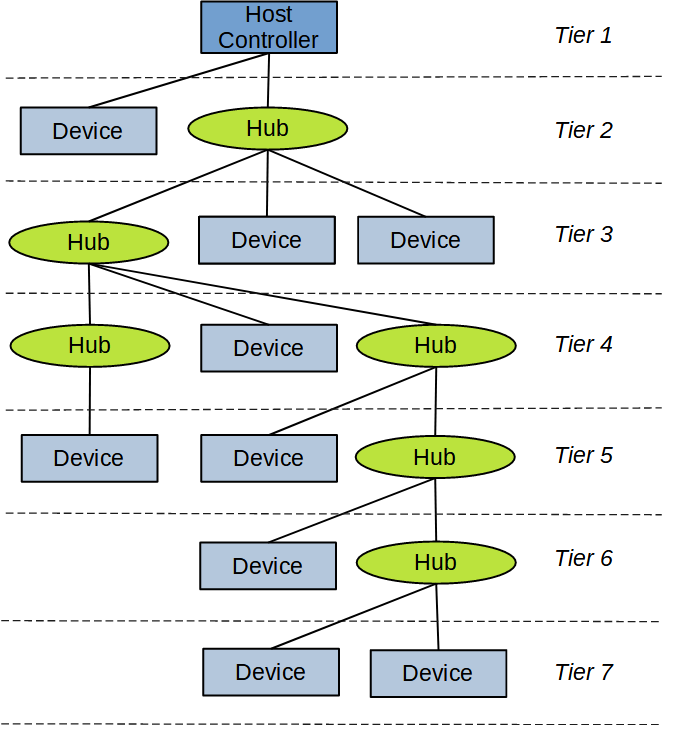
\includegraphics[scale=0.5]{DocuResources/usb_physical_topology.png}
    \end{center}
\end{figure}

\begin{itemize}
    \item Three types of USB Host controller.
    \item OHCI (Open Host Controller Interface)
          \begin{itemize}
              \item Compaq, Microsoft and National Semiconductors cooperated to produce this standard host controller specification for USB 1.0 and USB 1.1.
              \item Hardware Oriented
              \item Low speed and full Speed
          \end{itemize}
    \item UHCI (Universal Host Controller Interface)
          \begin{itemize}
              \item Intel's software-orientd of controller for USB 1.0 and 1.1
              \item Requieres license from Intel
              \item Low speed and full Speed
          \end{itemize}
    \item EHCI (Extended Host Controller Interface)
          \begin{itemize}
              \item USB 2.0 with high speed for a single host controller specs.
              \item EHCI handless high speed and hands off low and full speed to either OHCI or UHCI.
          \end{itemize}
    \item Four Wiere - VBUS [Red] (5V) , GND [Black] (reference), D+ [Green], D- [White]
    \item Carry differential data signal or single-ended signal states.
    \item The D+ or D- resistor should, strictly speaking, be pulled up to a 3.3V supply derived from Vbus, or controlled by Vbus in such a way that the resistor never sources current to the data line when Vbus is switched off.
\end{itemize}



\subsection{SPeed Identification}
\begin{itemize}
    \item At device end, a 1.5 kohm resistor pulls one of the lines to 3.3V supply derived from VBUS.
    \item Low speed : D- has the pull up resistor
    \item Full speed : D+ has the pull up resistor
    \item High speed : D+ has the pull up resistor
    \item host determine the speed by observering the lines.
\end{itemize}

\subsection{Transceivers}
\begin{itemize}
    \item Transceivers differe mainly by resistors.
    \item Upstream is the host end, where a 15k pull down resistor pulls the line low.
    \item Maximum high-leve is 3.3V
\end{itemize}
\begin{figure}[H]
    \begin{center}
        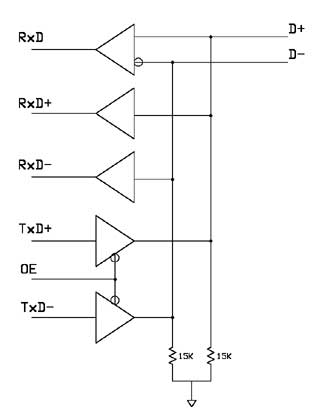
\includegraphics[scale=0.5]{DocuResources/TransceiversUp.jpg}
        \caption{Upstream Host Transceiver}
    \end{center}
\end{figure}
\begin{itemize}
    \item Downstream is at device end, where eithere there is a pull up resistor of 1.5kOhm at D+ or D- to make then high.
    \item Can be able to detect states (such as SE0 - both lines are low)
\end{itemize}
\begin{figure}[H]
    \begin{center}
        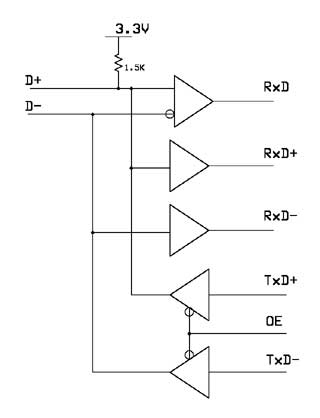
\includegraphics[scale=0.5]{DocuResources/TransceiversDOwn.jpg}
        \caption{Downstream device Transceiver (Full Speed)}
    \end{center}
\end{figure}

\subsection{Line States}
Based the 2 data lines, different line states are obtained.

\subsubsection{Detached}
When no device is plugged in, the host will see line low due to 15kohm pulling the lines low.
\begin{center}
    \begin{tikztimingtable}[%
            timing/dslope=0.1,
            timing/.style={x=5ex,y=2ex},
            x=5ex,
            timing/rowdist=3ex,
            timing/c/rising arrows,
            timing/name/.style={font=\sffamily\scriptsize}
        ]
        \busref{D+}   & X{}; 12L;\\
        \busref{D-} & X{}; 12L;\\
    \end{tikztimingtable}
\end{center}
\subsubsection{Attached}
Either of D+ or D- goes to high level to indicated the device is plugged in.

\begin{figure}[H]
    \begin{center}
        \begin{tikztimingtable}[%
                timing/dslope=0.1,
                timing/.style={x=5ex,y=2ex},
                x=5ex,
                timing/rowdist=3ex,
                timing/c/rising arrows,
                timing/name/.style={font=\sffamily\scriptsize}
            ]
            \busref{D+}   & X{}; L; 11H;\\
            \busref{D-} & X{}; 12L;\\
        \end{tikztimingtable}
    \end{center}
    \caption{Full SPeed}
\end{figure}

\begin{figure}[H]
    \begin{center}
        \begin{tikztimingtable}[%
                timing/dslope=0.1,
                timing/.style={x=5ex,y=2ex},
                x=5ex,
                timing/rowdist=3ex,
                timing/c/rising arrows,
                timing/name/.style={font=\sffamily\scriptsize}
            ]
            \busref{D+}   & X{}; 12L;\\
            \busref{D-} & X{}; L; 11H;\\
        \end{tikztimingtable}
    \end{center}
    \caption{Low SPeed}
\end{figure}

\subsubsection{Idle}
When the pulled up line is high and other line is low.
State of lines before and after packets are sent.
\begin{figure}[H]
    \begin{center}
        \begin{tikztimingtable}[%
                timing/dslope=0.1,
                timing/.style={x=5ex,y=2ex},
                x=5ex,
                timing/rowdist=3ex,
                timing/c/rising arrows,
                timing/name/.style={font=\sffamily\scriptsize}
            ]
            \busref{D+}   & X{};  12H;\\
            \busref{D-} & X{}; 12L;\\
        \end{tikztimingtable}
    \end{center}
    \caption{Full SPeed}
\end{figure}

\begin{figure}[H]
    \begin{center}
        \begin{tikztimingtable}[%
                timing/dslope=0.1,
                timing/.style={x=5ex,y=2ex},
                x=5ex,
                timing/rowdist=3ex,
                timing/c/rising arrows,
                timing/name/.style={font=\sffamily\scriptsize}
            ]
            \busref{D+}   & X{}; 12L;\\
            \busref{D-} & X{}; 12H;\\
        \end{tikztimingtable}
    \end{center}
    \caption{Low SPeed}
\end{figure}



\subsubsection{J and K State}
J state is same as Idle state, but the lines are driven by eigher host or device.
Opposite to J state.
J and K are used for full and low speed links as they are Opposite polarity.
\begin{figure}[H]
    \begin{center}
        \begin{tikztimingtable}[%
                timing/dslope=0.1,
                timing/.style={x=5ex,y=2ex},
                x=5ex,
                timing/rowdist=3ex,
                timing/c/rising arrows,
                timing/name/.style={font=\sffamily\scriptsize}
            ]
            \busref{D+}   & X{};  12H;\\
            \busref{D-} & X{}; 12L;\\
        \end{tikztimingtable}
    \end{center}
    \caption{J state}
\end{figure}

\begin{figure}[H]
    \begin{center}
        \begin{tikztimingtable}[%
                timing/dslope=0.1,
                timing/.style={x=5ex,y=2ex},
                x=5ex,
                timing/rowdist=3ex,
                timing/c/rising arrows,
                timing/name/.style={font=\sffamily\scriptsize}
            ]
            \busref{D+}   & X{}; 12L;\\
            \busref{D-} & X{}; 12H;\\
        \end{tikztimingtable}
    \end{center}
    \caption{K state}
\end{figure}

\subsubsection{SE0 state (Single Ended Zero)}
Both lines are pulled low.
Driven low.
\begin{figure}[H]
    \begin{center}
        \begin{tikztimingtable}[%
                timing/dslope=0.1,
                timing/.style={x=5ex,y=2ex},
                x=5ex,
                timing/rowdist=3ex,
                timing/c/rising arrows,
                timing/name/.style={font=\sffamily\scriptsize}
            ]
            \busref{D+}   & X{};  12L;\\
            \busref{D-} & X{}; 12L;\\
        \end{tikztimingtable}
    \end{center}
\end{figure}

\subsubsection{SE1 state (Single Ended One)}
Both lines are high.
Illegal, not happen.
\begin{figure}[H]
    \begin{center}
        \begin{tikztimingtable}[%
                timing/dslope=0.1,
                timing/.style={x=5ex,y=2ex},
                x=5ex,
                timing/rowdist=3ex,
                timing/c/rising arrows,
                timing/name/.style={font=\sffamily\scriptsize}
            ]
            \busref{D+}   & X{};  12H;\\
            \busref{D-} & X{}; 12H;\\
        \end{tikztimingtable}
    \end{center}
\end{figure}

\subsubsection{Reset}
When host wants to communicate it will start by applying Reset condition, which will set device to default config.
\begin{itemize}
    \item Pulling down lines to low for 10 ms (SE0 state)
    \item Device may recognie reset after 2.5 $\mu$s
\end{itemize}

\begin{figure}[H]
    \begin{center}
        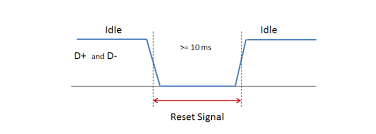
\includegraphics[scale=0.5]{DocuResources/resetSingal.png}
    \end{center}
\end{figure}

\subsubsection{EOP - ENd of Pack}
EOP is SE0 for 2 bit time, and J state for 1 bit time.
\begin{figure}[H]
    \begin{center}
        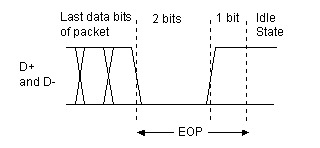
\includegraphics[scale=0.5]{DocuResources/EOPSignal.jpg}
    \end{center}
\end{figure}

\subsubsection{Suspend}
Not sending any signal for 3 ms. (IDLE state)
Normally a SOF packet (at full speed) or a Keep Alive signal (at low speed) is sent by the host every 1 ms, and this is what keeps the device awake.
\begin{figure}[H]
    \begin{center}
        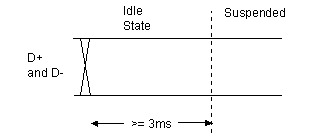
\includegraphics[scale=0.5]{DocuResources/SuspendSIgnal.jpg}
    \end{center}
\end{figure}


\subsubsection{Resume}
Wake up device which is in suspend.
Reverse the polarity of the lines for atlease 20ms.
Followed by low speed EOP signal.

\begin{figure}[H]
    \begin{center}
        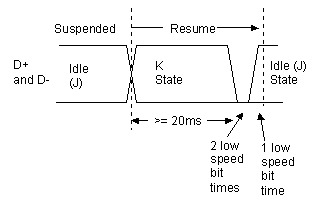
\includegraphics[scale=0.5]{DocuResources/resumesignal.jpg}
    \end{center}
\end{figure}

\subsubsection{Keep Alive signal}
Low speed EOP.
Atleaset every 1ms on low speed link to keep the device from suspending.
\begin{figure}[H]
    \begin{center}
        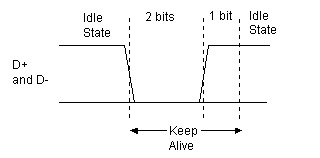
\includegraphics[scale=0.5]{DocuResources/KEEPAlige.jpg}
    \end{center}
\end{figure}

\subsection{Packets and Transmission}
\begin{itemize}
    \item Packets - smallest element of data transmission.
    \item Before and after Packet, the bus is idle.
    \item \textcolor{red}{\textbf{Serial Interface Engine (SIE)} takes care of SYNCs, Bit Stuffing, and EOP conditoions}.
    \item USB uses LSB first. (also in a 2-byte data, LSB byte is transmitted first)
    \item Packets starts with a SYNC pattern to synchronize with the receiver bit clock.
    \item Followed by data packets and ends with EOP signal.
    \item NRZI encoding
    \item to ensure sufficent frequent transitions - Bit Stuffing (zero after 6 sucessive 1's) is done.
\end{itemize}


\subsection{Definitions}
\subsubsection{EndPoints}
\begin{itemize}
    \item Each USB device has a number of endpoints.
    \item Each endpoint is a source or a sink of data.
    \item A device can have upto 16 OUT and 16 IN endpoints
    \item OUT means from host to device.
    \item IN means device to host.
    \item Endpoint 0 is combination of endpoint0 OUT and endpoint0 IN and is used for controlling device.
\end{itemize}

\subsubsection{Pipes}
\begin{itemize}
    \item A logical connection between host and a particular endpoint.
\end{itemize}

\subsubsection{Transactions}
\begin{itemize}
    \item Simple transfer of data called Transactions built up using packets.
\end{itemize}



\subsection{Packet FOrmat}
\begin{itemize}
    \item The first byte of every packet is the Packet Identifier (PID).
    \item To make it easy for the SIE, there is no CRC check for PID.
    \item USB uses two CRCs - 5-bit CRC (CRC5) and 16-bit CRC (CRC16)
    \item First two bits of PID determines the groups in which they fall into.
    \item Even Here LSB's are transmitted first, hence, PID0 is transmitted first, followed by PID1, PID2, PID3, $\overline{PID0}$, $\overline{PID1}$, $\overline{PID2}$, $\overline{PID3}$
\end{itemize}

\begin{bytefield}[bitformatting={\large\bfseries},
        endianness=little,bitwidth=0.1\linewidth]{8}
    \bitlabel{1}{LSB}
    \bitlabel{13}{MSB}\\
    \bitbox{1}{\small PID0}
    \bitbox{1}{\small PID1}
    \bitbox{1}{\small PID2}
    \bitbox{1}{\small PID3}
    \bitbox{1}{\small  $\overline{PID0}$}
    \bitbox{1}{\small  $\overline{PID1}$}
    \bitbox{1}{\small  $\overline{PID2}$}
    \bitbox{1}{\small  $\overline{PID3}$}\\
\end{bytefield}

\subsubsection{Token Packet}
\begin{bytefield}[bitformatting={\large\bfseries},
        endianness=little,bitwidth=0.1\linewidth]{6}
    \bitlabel{1}{SYNC}
    \bitlabel{1}{PID}
    \bitlabel{1}{ADDR}
    \bitlabel{1}{ENDP}
    \bitlabel{1}{CRC5}
    \bitlabel{1}{EOP}\\
    \bitbox{1}{}
    \bitbox{1}{\small 8 bits}
    \bitbox{1}{\small 7 bits}
    \bitbox{1}{\small 4 bits}
    \bitbox{1}{\small  5 bits}
    \bitbox{1}{}\\
\end{bytefield}
\begin{itemize}
    \item User for SETUP, OUT, IN packets.
    \item Transmitted first in a transaction - identify the endpoint and purpose of transacting.
    \item Address is 7-bit can so can address upto 127 adddressed using USB (Address 0 is reserved).
    \item Endpoint can be upto 16-possible values in each directions(IN or OUT).
    \item The direction (IN or OUT) is said by PID.
          \begin{itemize}
              \item OUT and SETUP PID will refer OUT endpoint.
              \item IN PID will refere IN endpoint.
          \end{itemize}
\end{itemize}


\subsubsection{Data Packets}
\begin{bytefield}[bitformatting={\large\bfseries},
        endianness=little,bitwidth=0.12\linewidth]{5}
    \bitlabel{1}{SYNC}
    \bitlabel{1}{PID}
    \bitlabel{1}{DATA}
    \bitlabel{1}{CRC16}
    \bitlabel{1}{EOP}\\
    \bitbox{1}{}
    \bitbox{1}{\small 8 bits}
    \bitbox{1}{\small (0-1024) $\times$ 8 bits}
    \bitbox{1}{\small 16 bits}
    \bitbox{1}{}\\
\end{bytefield}
\begin{itemize}
    \item Used for DATA0, DATA1, DATA2, MDATA packet.
    \item For data stage inside a transaction.
    \item DIfferent DATA for error-checkng system.
    \item DATA0 and DATA1 is used in Low and FUll speed links.
          \begin{itemize}
              \item DATA0 and DATA1 packets comes alternatively when sending data.
              \item This helps endpoint to know which one to expect.
          \end{itemize}
    \item DATA2 and MDATA are used for high speed links.
\end{itemize}

\subsubsection{Handshake Packet}
\begin{bytefield}[bitformatting={\large\bfseries},
        endianness=little,bitwidth=0.12\linewidth]{3}
    \bitlabel{1}{SYNC}
    \bitlabel{1}{PID}
    \bitlabel{1}{EOP}\\
    \bitbox{1}{}
    \bitbox{1}{\small 8 bits}
    \bitbox{1}{}\\
\end{bytefield}

\begin{itemize}
    \item USed for ACK, NAK, STALL, NYET.
    \item status stage of a transcation.
    \item ACK - reciever acknowledges error free packet.
    \item NACK - receiver cannot accept data or tranmitting device cannot send data.
    \item STALL - endpoint is halted
    \item NYET - No response yet from receiver (high speed only)
\end{itemize}


\subsubsection{SOF Packet}
\begin{bytefield}[bitformatting={\large\bfseries},
        endianness=little,bitwidth=0.1\linewidth]{5}
    \bitlabel{1}{SYNC}
    \bitlabel{1}{PID}
    \bitlabel{1}{Frame No.}
    \bitlabel{1}{CRC5}
    \bitlabel{1}{EOP}\\
    \bitbox{1}{}
    \bitbox{1}{\small 8 bits}
    \bitbox{1}{\small 11 bits}
    \bitbox{1}{\small  5 bits}
    \bitbox{1}{}\\
\end{bytefield}
\begin{itemize}
    \item Only on full speed links.
\end{itemize}


\subsection{Transactions}
\begin{itemize}
    \item A transaction (successfull) is a sequence of three packets which perform a simple transfer of data.
    \item For IN and OUT transaction used for isochronous transfers, only 2 tpackets are used, the handshake packet at the end is omitted.
    \item This is because error-checking is not required.
\end{itemize}
\begin{figure}[H]
    \centering
    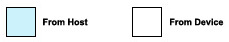
\includegraphics[]{DocuResources/TransactionIdea.jpg}
\end{figure}

\subsubsection{OUT Transaction}
\begin{itemize}
    \item A successfull OUT transaction comprises two or three sequential packets.
    \item FOr isochronous transfer, only two packets and handshake packet from the device is obmitted.
    \item On Low or full speed link, DATAx is either DATA0 or DATA1 alternating between them.
\end{itemize}

\begin{figure}[H]
    \centering
    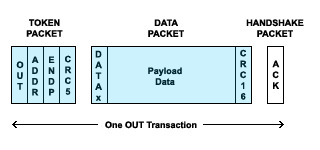
\includegraphics[]{DocuResources/OUTTrans.jpg}
\end{figure}

\subsubsection{IN Transaction}
\begin{itemize}
    \item A successfull IN transaction comprises two or three sequential packets.
    \item FOr isochronous transfer, only two packets and handshake packet from the host is obmitted.
    \item On Low or full speed link, DATAx is either DATA0 or DATA1 alternating between them.
\end{itemize}

\begin{figure}[H]
    \centering
    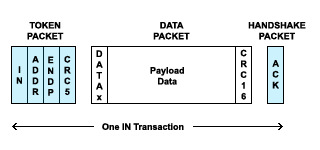
\includegraphics[]{DocuResources/INTrans.jpg}
\end{figure}

\subsubsection{SETUP Transaction}
\begin{itemize}
    \item A successfull IN transaction comprises three sequential packets.
    \item similar to OUT transaction, but data payload is exactly 8-bytes long.
    \item SETUP PID in token packet tells the de4vice thiat this is the first transaction in COntrol transfer.
    \item SETUP transaction always use DATA0
\end{itemize}

\begin{figure}[H]
    \centering
    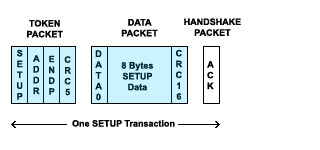
\includegraphics[]{DocuResources/SETUPtrans.jpg}
\end{figure}

\subsection{Data Flow Types}
\begin{itemize}
    \item Four Different ways to transfer data on a USB bus.
    \item Each has its own purpose and characteristics.
    \item Each one is built up using one or more transaction type.
\end{itemize}


\subsubsection{Bulk Transfers}
\begin{itemize}
    \item Transfer large amounts of data with error-free but no guanrantee of bandwidth.
    \item Host will \textit{schedule} bulk transfers after other transfer types have been allocated.
    \item If an OUT endpoint is defined as using Bulk transfers, then the host will transfer data to it using OUT transactions.
    \item If an IN endpoint is defined as using Bulk transfers, then the host will transfer data from it using IN transactions.
    \item The max packet size is 8, 16, 32 or 64 at full Speed and 512 for high speed.
    \item Bulk transfers are not allowed at low speed.
    \item See topic : Bulk Transfers on more details if needed.
\end{itemize}

Shown below is a Bulk transfer of OUT transactions in OUT endpoint.
\begin{figure}[H]
    \centering
    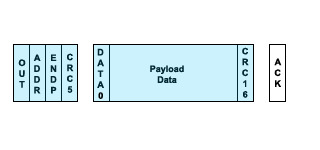
\includegraphics[]{DocuResources/BulkOUTTrans.jpg}
\end{figure}

\subsubsection{Interrupt Transfer}
\begin{itemize}
    \item Regularly scheduled IN or OUT transactions. (mosly IN directions)
    \item Host fetches one packet from device at an interval specifed by the endpoint descriptor.
    \item Use an interrupt transfer when you need to be regularly kept up to date of any changes of status in a device.
\end{itemize}

\begin{figure}[H]
    \centering
    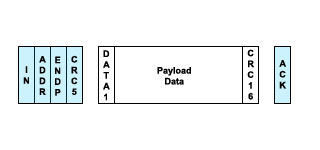
\includegraphics[]{DocuResources/InterruptINTransfer.jpg}
\end{figure}

\subsubsection{Isochronous Transfers}
\begin{itemize}
    \item Guaranteed bandwith, but no error-free.
    \item Applications of audio data transfer.
    \item either an In or OUT transcation depending on the type of endpoint.
    \item No need handshake packet at the last.
    \item may containe upto 1023 bytes at full speed.
    \item 1024 at high speed.
    \item No transfer at low speed.
\end{itemize}

Shown below, is a isochronous transfer of IN transaction.
\begin{figure}[H]
    \centering
    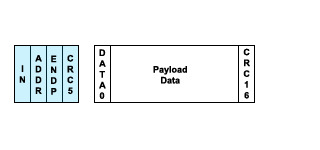
\includegraphics[]{DocuResources/IsochrnousINTransfer.jpg}
\end{figure}

\subsubsection{Control Transfer}
\begin{itemize}
    \item Bi-direction transfer which uses both IN and OUT endpoint.
    \item Each control transfer must have 2 or more transaction (the 2 transactions beeting SETUP stage (SETUUP/OUT transaction) and STAUTS stage )
    \item Has three stages.
          \begin{itemize}
              \item SETUP stage carries 8 bytes called the setup packet.
              \item defines the request and specfies how much data should be transffered in DATA stage.
              \item DATA stage is optional,
              \item But if data stage is preset , it starts with DATA1 and alternates between DATA0 and DATA1. untill all data is transffered.
              \item The STAUS stage is a transaction containing a zero-lenght DATA1 packet.
              \item If DATA  stage was IN, then STATUS stage is OUT and vice versa.
          \end{itemize}
    \item Control transfers are used for initial configuration of the device by the host.
    \item Uses the Endpoint 0 OUT and Endpoint 0 IN.
\end{itemize}

Shown below is a control transfer with data stage as IN.
\begin{figure}[H]
    \centering
    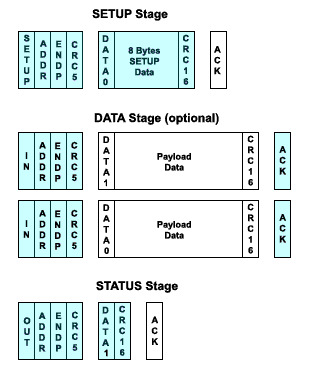
\includegraphics[]{DocuResources/ControlINtransfer.jpg}
\end{figure}


\subsection{Controlling Device}
\begin{itemize}
    \item When USB devices is plugged in, the host becomes aware that a device is plugged in ( because of the pull resistor on one of the data lines)
    \item The host now signals a USB reset to the device to makes the device enter a known state at the end of reset.
    \item In reset state, the device responds to default address of 0.
    \item Now, the host will sedn a request to \textbf{Endpoint 0} with device address 0 to find out its maximum packet size.
    \item It can discover this using \verb|Get_Desriptor| command.
    \item The device responds on address 0.
    \item The host now will reset the device again.
    \item Then it sends a \verb|Set_Address| request with adress 0.
    \item After request is complete, the devices assumes the new address.
    \item Now, the host gets details from the device using the
          \begin{itemize}
              \item \verb|Get_Device| Descriptor
              \item \verb|Get_Configuration| Descriptor
              \item \verb|Get_String| Descriptor
          \end{itemize}
    \item Once, the host gets the enough details, the host loads the suitable device driver.
    \item The device driver will then select a configuration for the device by sending a \verb|Set_Configuration| request to device.
    \item Now, the device is in configured state.
    \item Now, it can respond to device specific request.
    \item THese are done using Control transfers on Endpoint 0 IN and OUT.
\end{itemize}



\end{document}
